\chapter{Theory Literature Review}
\label{chp:TheoryLit}
This chapter will accumulate a thorough understanding of the theory and current state of technology relevant to the measurement of each medical sign required of the Ear-Monitor. Attention will be given to the different methods available to determine each medical sign. This section will also make reference to various articles and studies done by other researchers in this field of study. The aim is to gather all the relevant information in order to make an informed selection of the methods and sensors the Ear-Monitor will use to measure each medical sign.

\section{Core Temperature}
Various methods are available for measuring core temperature. Non-electric, fluid-filled thermometers was the first to be used. The mercury-filled thermometer was used by early physicians to study the thermoregulation of the human body and crudely identify fevers. Since then, the mercury has been replaced by coloured alcohol or another heat sensitive liquid, due to toxicity of mercury.

\medskip

Another type of fluid-filled thermometer is the liquid-crystal thermometer. It contains liquid crystals that changes colour when at different temperatures. The use of these two types of fluid-filled thermometers has decreased significantly due to the accuracy, speed and connivance of digital thermometers.

\medskip

Electrical thermometers are now the industry standard of measuring core temperature. Central to any digital thermometer lies a transducer that convert temperature to an electrical signal. Resistance temperature detectors, thermocouples thermistor and thermopiles will be discussed. They can be divided into contact and non-contact thermometers.

\subsection{Contact Thermometers}
These are a family of thermometers that measure their own temperature with the assumption they and the object whose temperature is of interest, are in thermal equilibrium. Therefore, they are usually placed in contact with the object. When using a contact thermometer in the ear, the sensor part of the thermometer can be placed in contact with the ear canal wall, the air inside the canal or with the tympanic membrane self.

\subsubsection{Resistance Temperature Detector}

Resistance temperature detectors (RTDs) uses the temperature-resistance relationship for metals to measure temperature. Thin wire coils or films of platinum, copper or nickel are usually preferred for they have a stable and repeatable temperature-resistance relationship over a large temperature range.

\subsubsection{Thermocouple}
Thermocouples make use of the thermo-electric effect to make a temperature measurement. They consist of two dissimilar conductors connected at the one end, knows as the hot junction (measuring junction). The other ends of the two wires are known as the cold junction (reference junction) and are connected to a voltage meter via common conductors. A voltage is generated dependant to the temperature difference between the measuring- and reference junctions. Thermocouples do not respond to absolute temperature; therefore, their accuracy depends on how well the reference temperature can be defined. Reference temperatures are usually determined by a precise thermistor. Thermocouples are very versatile and widely used in clinical applications, but the downsides are that their output signal is low and non-linear, therefore requiring a sensitive and stable voltage measuring device \citep{jones2010biomedical}.

\medskip

Thermocouples can be connected in series and are then called thermopiles. This configuration sums the output voltages, resulting in temperature averaging. This method improves accuracy by reducing noise. 

\subsubsection{Thermistor}
A thermistor is a type of semiconductor whose resistance varies with changes in temperature. They differ from RTDs in that they are usually made of ceramics, they have higher precision over a smaller temperature range and they can have a negative relation to temperature. Thermistors are preferred above RTDs and thermocouples for use as biomedical sensors due to their faster response time and higher sensitivity over a smaller range and. The smaller range does not matter, for the temperature range of interest in biosensors are small and well defined. 

\subsubsection{Contact Thermometer Application}
In the case of RTDs and thermistors, the measuring element is placed in position and a current is sent through the sensor. By measuring the voltage across the resistive element, it is possibly to calculate the voltage and subsequently determine the temperature. In the case of the thermocouple, the hot junction can be placed in contact with the canal wall or tympanum. Typically, the hot junction will be enclosed with a soft material to protect the canal and tympanum. The canal is sealed off and time is allowed for the area to equilibrate to tympanic temperature.

\medskip

Placing a thermometer in contact with the tympanic membrane will give an accurate measurement, but can cause discomfort to the wearer. There is also a risk of harming the tympanic membrane. Sensors in contact with the ear canal wall or the air inside the canal run the risk of making errors by measuring the temperature of objects that are not in thermal equilibrium with the tympanic membrane. Therefore, non-contact thermometers will be considered.

\subsection{Non-contact Thermometers}
Thermopiles can be used to detect thermal radiation without being I contact with the object. All matter with temperatures above 0 K radiates electromagnetic radiation according to the Stefan-Boltzman law. The thermal radiation, $Q$, per unit area is given by the equation:

$$Q=\varepsilon \sigma T^4.$$

Where $\varepsilon$ is the emissivity, $\sigma$ the Stefan-Boltzman constant and T the temperature of the object.

The wavelength distribution varies according to the temperature of the object and is described by Planck's law:

$$B_\lambda (\lambda ,T)=\frac{2hc^2}{\lambda ^5}\frac{1}{e^\frac{hc}{\lambda k_B T} -1}.$$
 
Where $B_\lambda$ is the spectral radiance, $\lambda$ the radiation wavelength, $h$ Planck's constant, $k_B$ Boltzman's constant $c$ the speed of light and $T$ the object's temperature. Through maximizing $B_\lambda$ , it is possible to find the dominant wavelength that is emitted at a certain temperature. Figure~\ref{fig:PlancksLaw} shows a plot made of spectral radiance versus wavelength at $T=$ 37 $^{\circ}C$, the core temperature of humans. It can be seen that the dominant wavelength is at 9.35 $\mu$m. This is in the infrared range, and therefore this type of thermal radiation thermometer is called an infrared thermometer.

\medskip

 \begin{figure}[h]
   \centering
   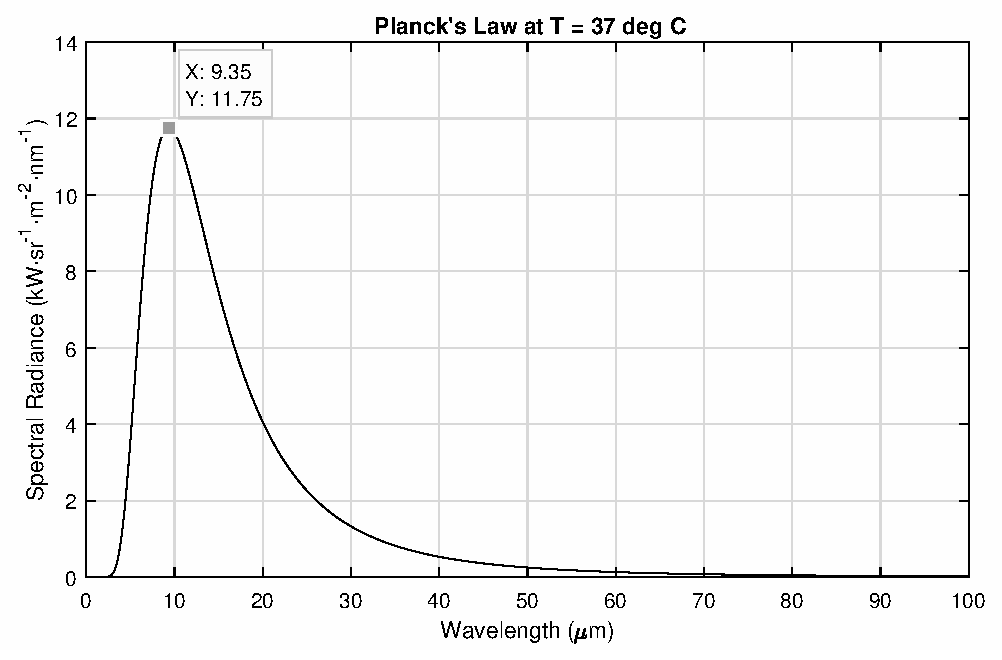
\includegraphics[scale=0.6]{figs/PlancksLaw}
   \caption{Plot showing how Planck's law can be used to determine the dominant radiation wavelength at certain temperature}
   \label{fig:PlancksLaw}
\end{figure}

In the case of measuring the temperature of the tympanic membrane, the hot junction's temperature will be determined by the radiation received from the tympanum minus the radiation radiated by the sensor self.

\medskip

When talking about thermal radiation, an important aspect is emissivity. Emissivity is the ability of an object to radiate thermal energy. It is quantified as a ratio of thermal energy emitted by a surface relative to the thermal energy emitted by an ideal black body at the same temperature. A black body is an idealized surface that reflects no radiation, meaning all energy radiated from the surface are due to the temperature of the surface. Thus, a black body have an emissivity of 1 and have the maximum theoretical radiation at a given temperature. The accuracy of an infrared sensor depends on the ability of the object to emit sufficient thermal radiation for the sensor to detect. Cross-referencing various emissivity tables, it was found that the emissivity of human skin is 0.98, meaning that it is an excellent emitter of thermal energy \citep{stumme2003emissivity} \citep{EmissivityThermoWorks} \citep{EmissivityOptotherm}. The ear drum is covered with skin, making it an ideal target object for a non-contact thermometer.

\medskip

An infrared thermometer generally consists out of a thermophile attached to a blackbody and shielded by an infrared filter that also acts as a lens to focus infrared waves \citep{irTempSensors}. This setup, shows in Figure \ref{fig:IR_Thermometer}, allows for the non-contact temperature sensing of the tympanic membrane. Unlike pulse rate, breathing and electrical brain activity, the core body temperature varies slowly. It takes minutes to vary significantly. Therefore, the sampling period of core temperature can be as long as 10 seconds.

\medskip

\begin{figure}
   \centering
   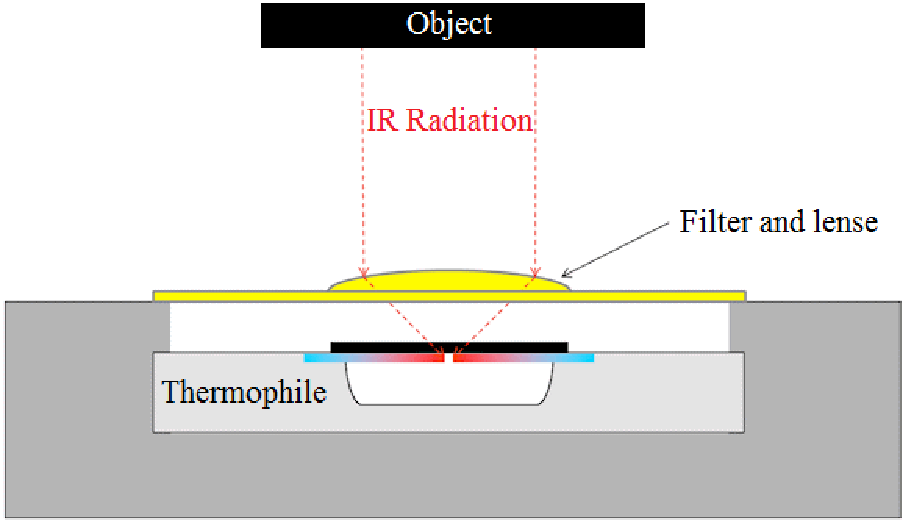
\includegraphics[scale=0.5]{figs/IR_Thermometer}
   \caption{IR Thermometer diagram (V Polyzoev et al: Demystifying Thermopile IR Temp Sensors)}
   \label{fig:IR_Thermometer}
\end{figure}

\subsection{Commercial Temperature Monitoring Devices}
Ear thermometers are widely used at home and in hospitals. Ear contact thermometers like Novatemp\textsuperscript \textregistered{} and Starboard\textsuperscript \textregistered{} claims a $\pm$0.2 $^{\circ}C$ accuracy. Non-contact infrared ear thermometers usually have a similar rated accuracy. None of these are, however, wearable devices. 

\medskip
 
The \textit{degree}$^{\circ}$, Figure \ref{fig:Degree}, is a continuous in-ear thermometer for children, developed by \textit{cosinuss}$^{\circ}$, a company specialising in wearable sensors. The bulk of the device is worn behind the ear, and there is a wire running over the auricle to the ear canal, in which a probe is placed. The device takes its temperature measurements with a sensor placed in contact with the canal wall. The manufacturer claims an accuracy of $\pm$0.1 $^{\circ}C$. It monitors temperature continuously and sends real time data to a mobile phone.

\medskip

\begin{figure}[h]
   \centering
   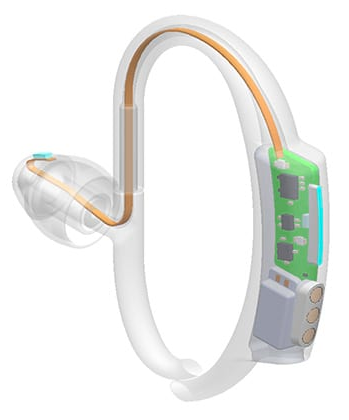
\includegraphics[scale=0.5]{figs/Degree}
   \caption{CAD model of the \textit{degree}$^{\circ}$ from the \textit{cosinuss}$^{\circ}$ website (include ref)}
   \label{fig:Degree}
\end{figure}

Apart from the \textit{degree}$^{\circ}$, there are not much literature on wearable ear thermometers. Two patents were found describing similar devices: US 6556852 B1 and US 20090221888 A1. The first of which proposes the use of an infrared sensor pointed at the tympanic membrane, and the latter not specifying the method of measuring. Hopefully, the tests planned for this study can add to this insufficient body of knowledge.

\section{Heart Rate}
The heart is a very dynamic organ whose influence can be felt throughout the body. Therfore there are many options available to monitor heart rate. Electronic monitoring methods include electrocardiography (ECG), photoplethysmography (PPG), ballistocardiography(BCG), phonocardiography and doppler flow-meters.

\subsection{Electrocardiography}
ECG is a recording of the electrical activity of the heart over a period of time. Electrical activity arise from the depolarization and repolarization of the heart muscle during the cardiac cycle. The most prominent electrical charge is the QRS complex, which corresponds to the ventricular depolarization and is visible on the electrocardiogram as a sharp peak in the millivolt range. ECG is the the recommended way of monitoring heart rate in most intensive care units. A cardiologist will use a 12 lead ECG with 10 electrodes placed in a specific configuration on the chest. Various wearable devices use ECG to measure heart rate. Fitness monitors normally uses a chest strap with electrodes to detect the heart's electrical activity. Studies have been done developing wearable ECG devices for clinical use.

\medskip
The latest in wearable ECG electrodes is the use of dry polymer-based materials \citep{wang2010wearable} or non-contact electrodes that can be place on top of clothing \citep{lin2013development}. This is an improvement above the standard conductive gels or adhesives and can be used repeatedly. But these electrods still needs to be place on the chest.

\medskip
An ear located ECG monitor have been developed by \cite{winokur2012wearable}. This device uses a single lead set-up with one electrode place on the mastoid bone behind the ear and a reference electrode placed on the neck. This configuration relies on the conductive properties of human tissue to carry electrical charges form the heart to the ear. They where able to used the electrocardiogram in conjunction with PPG and BCG to determine various heart intervals and track changes in mean arterial blood pressure. Figure \ref{fig:Winokur} shows \cite{winokur2012wearable}'s device and a plot of its electrocardiogram. No heart rate information was extracted.

\medskip

\begin{figure}[hb]
   \centering
   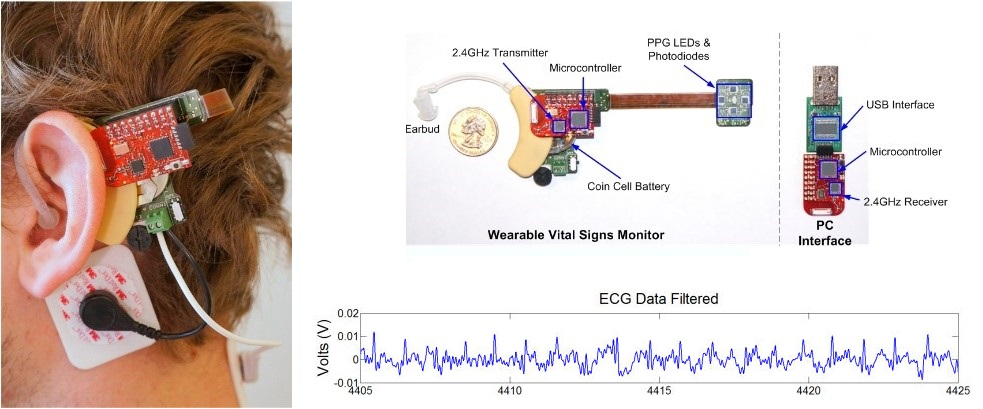
\includegraphics[scale=0.5]{figs/Winokur}
   \caption{Ear-worn device developed by \cite{winokur2012wearable}}
   \label{fig:Winokur}
\end{figure}

\subsection{Photoplethysmography}
PPG produces an optically obtained plethysmogram, which is a plot of volume the change of an organ over time. PPG can be used to measure the change in the volume of blood vessels close to the skin surface. When the left ventricle contracts a pressure pulse propagates through the arteries from the heart to the extremities of the body. This wave corresponds to the systolic blood pressure. Blood vessels walls contain elastic fibres that allow them to stretch. This means that the diameter of vessels will increase when the blood pressure increase, causing arteries to stretch and contract with each cardiac cycle. PPG can be used to determine heart rate by measuring this volumetric variation.

\medskip
A photoplethysmograph can non-invasively determine peripheral arterial blood volume by shining light through the skin surface, into the dermis and subcutaneous tissue and collecting the light transmitter or reflected. Light shined into the tissue can either be reflected, absorbed or allowed to transmit through. This leads to the two modes of PPG operation depicted by Figure \ref{fig:PPGModes}.

\medskip
 
\begin{figure}[h]
\centering
\graphicspath{{figs/}}
%\def\svgwidth{200pt}
\input{figs/PPGModes.pdf_tex}
\caption{The two modes of Photoplethysmography \citep{tamura2014wearable}}
\label{fig:PPGModes}
\end{figure}




In (a) the emitter and detector faces each other and are separated by tissue that can transmit the light, leading to a transmission mode PPG. Transmittance mode PPG is limited to locations on the body where transmitted light can be detected, like the finger, ear lobe, concha and tragus. These locations have limited blood profusion, especially at low temperatures. In (b) the emitter and detector is placed on the same plane and both faces toward the tissue. Light from the emitter is reflected by the tissue and captured by the detector, leading the reflection mode PPG. The emitter and collector needs to be optically isolated so that light cannot pass from the one to the other without going through the tissue. Reflectance mode PPG can be used at more locations, but they are more susceptible to motion artefacts \citep{tamura2014wearable}.

\medskip
According to Lambert's law, the amount of light absorbed is proportional to the length of the path that the light must travel in the absorbing substance \citep{lambertANDbeer}. Therefore, a change in blood vessel diameter will increase the distance the light must travel causing a change in light absorption. This can be detected by measuring reflected or transmitted light. Variation in the light reflected or transmitted will be synchronised with the heart rate.

\medskip
Shorter light wavelengths are mostly absorbed by the tissue, while longer wavelengths can penetrate deeper. Red and near infrared light are preferred for transmission PPG. While green light is becoming more popular for shallow reflectance PPG, due to larger light variations during the cardiac cycle and less noise than near infrared PPG \citep{tamura2014wearable}.

\medskip

The signal read by the photo detector of the pulse oximeter consists of a AC component superimposed on a DC signal. The DC component is the due to the constant transmission or reflection of light by the body's tissue: skin, fat, venous blood and the non-pulsating arterial blood. The AC components is the variation in transmitted or reflected light due to the change in diameter of the arteries and therefore, synchronised to the heart rate. The AC component is usually between 0.5 - 2\% of the DC component \citep{tavakoli2006analog}. Figure \ref{fig:PPG} illustrates the way in which which the heart rate is visible in a photoplethysmograph. It can be seen that the blood volume increase with each heartbeat, and that this causes more light to be absorbed, thus less detected by the photodiode.

\medskip

\begin{figure}[h]
   \centering
   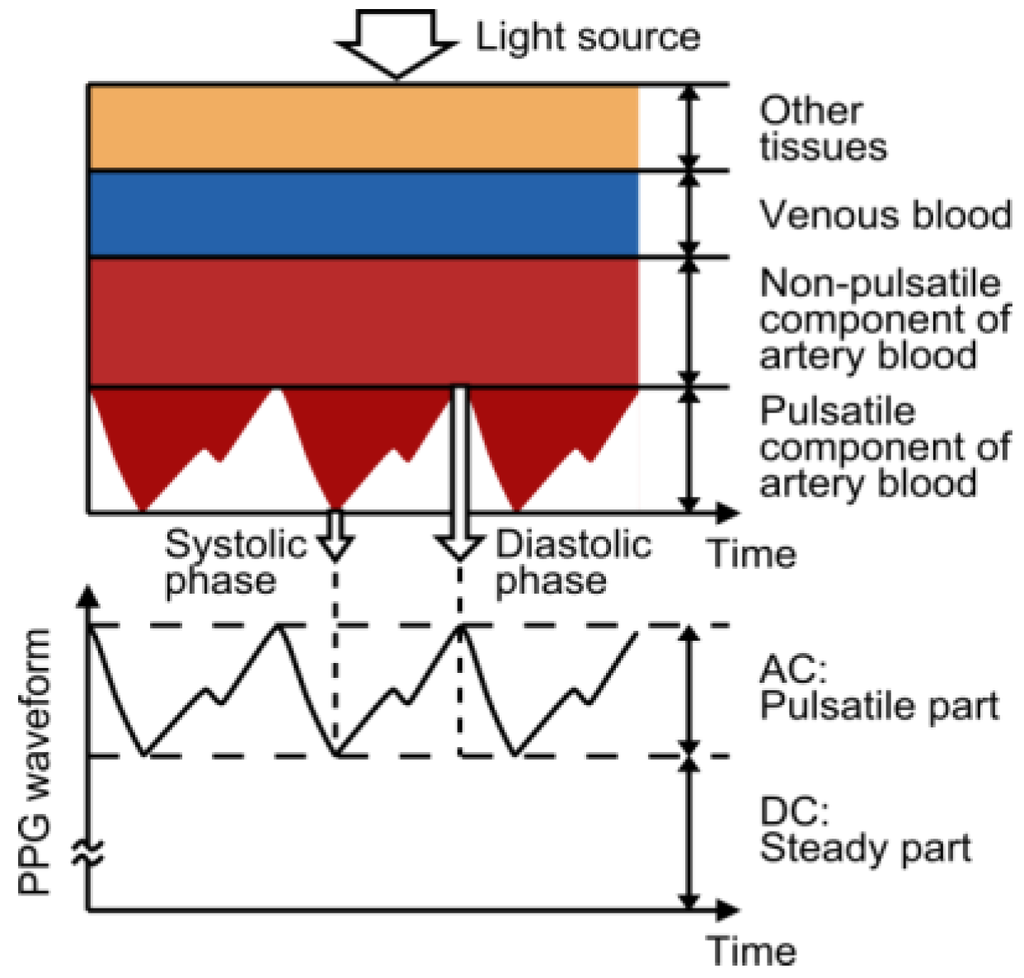
\includegraphics[scale=1.6]{figs/PPG}
   \caption{Dasic operating principles of PPG \citep{tamura2014wearable}}
   \label{fig:PPG}
\end{figure}

\subsubsection{Work done by others in Ear PPG}
At this point, PPG is the most attractive option for the Ear-Monitor to measure heart rate and it is given extra attention during the literature review.  A review of work done by others in the field of ear PPG revealed six devices relevant to this study.

\medskip
\cite{shin2009novel} presents a wearable music headset with an integrated transmission PPG ear clip that attaches to the ear lobe. The device includes an accelerometer to aid in the removal of motion artefacts. Evaluation was done through a study comparing the HR from the devise to that made with a conventional ECG recorder. This study revealed a heart rate error of 0.6\% was found.

\medskip
\cite{poh2010motion} designed a wearable PPG with a magnetic earring sensor. The bulk of device sits in front ear canal and held in place by the auricle. A reflective PPG sensor is held against the ear lobe by placing a magnet on the opposite side. The device also includes an accelerometer to make baseline measurements for motion artefact cancellation. A study was conducted to compare the PPG signals measured by the wearable device to chest ECG signals collected by a FDA-approved commercial system. Whilst standing motionless, the study found a very high agreement between the ear PPG and the chest ECG with a mean bias of 0.62 $\pm$ 4.51\% with ECG reference measurements.

\medskip

\begin{figure}[h]
   \centering
   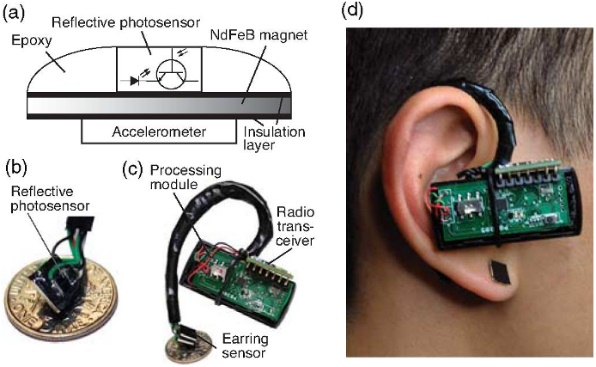
\includegraphics[scale=1.2]{figs/poh}
   \caption{Pulse oximetry diagram \citep{poh2010motion}}
   \label{fig:poh}
\end{figure}

\cite{da2010ear} researched an ear worn heart rate monitor containing PPG sensor in reflectance mode. Red light is shined into the tissue behind the ear and collected by a photodiode chip with an integrated transimpedance amplifier. Signals were not digitalised on the device, but recorded and processed on MATLAB. They compared their collected signal with a transition finger PPG and a chest ECG. Figure \ref{fig:DaHe} shows this comparison.

\medskip

\begin{figure}[h]
   \centering
   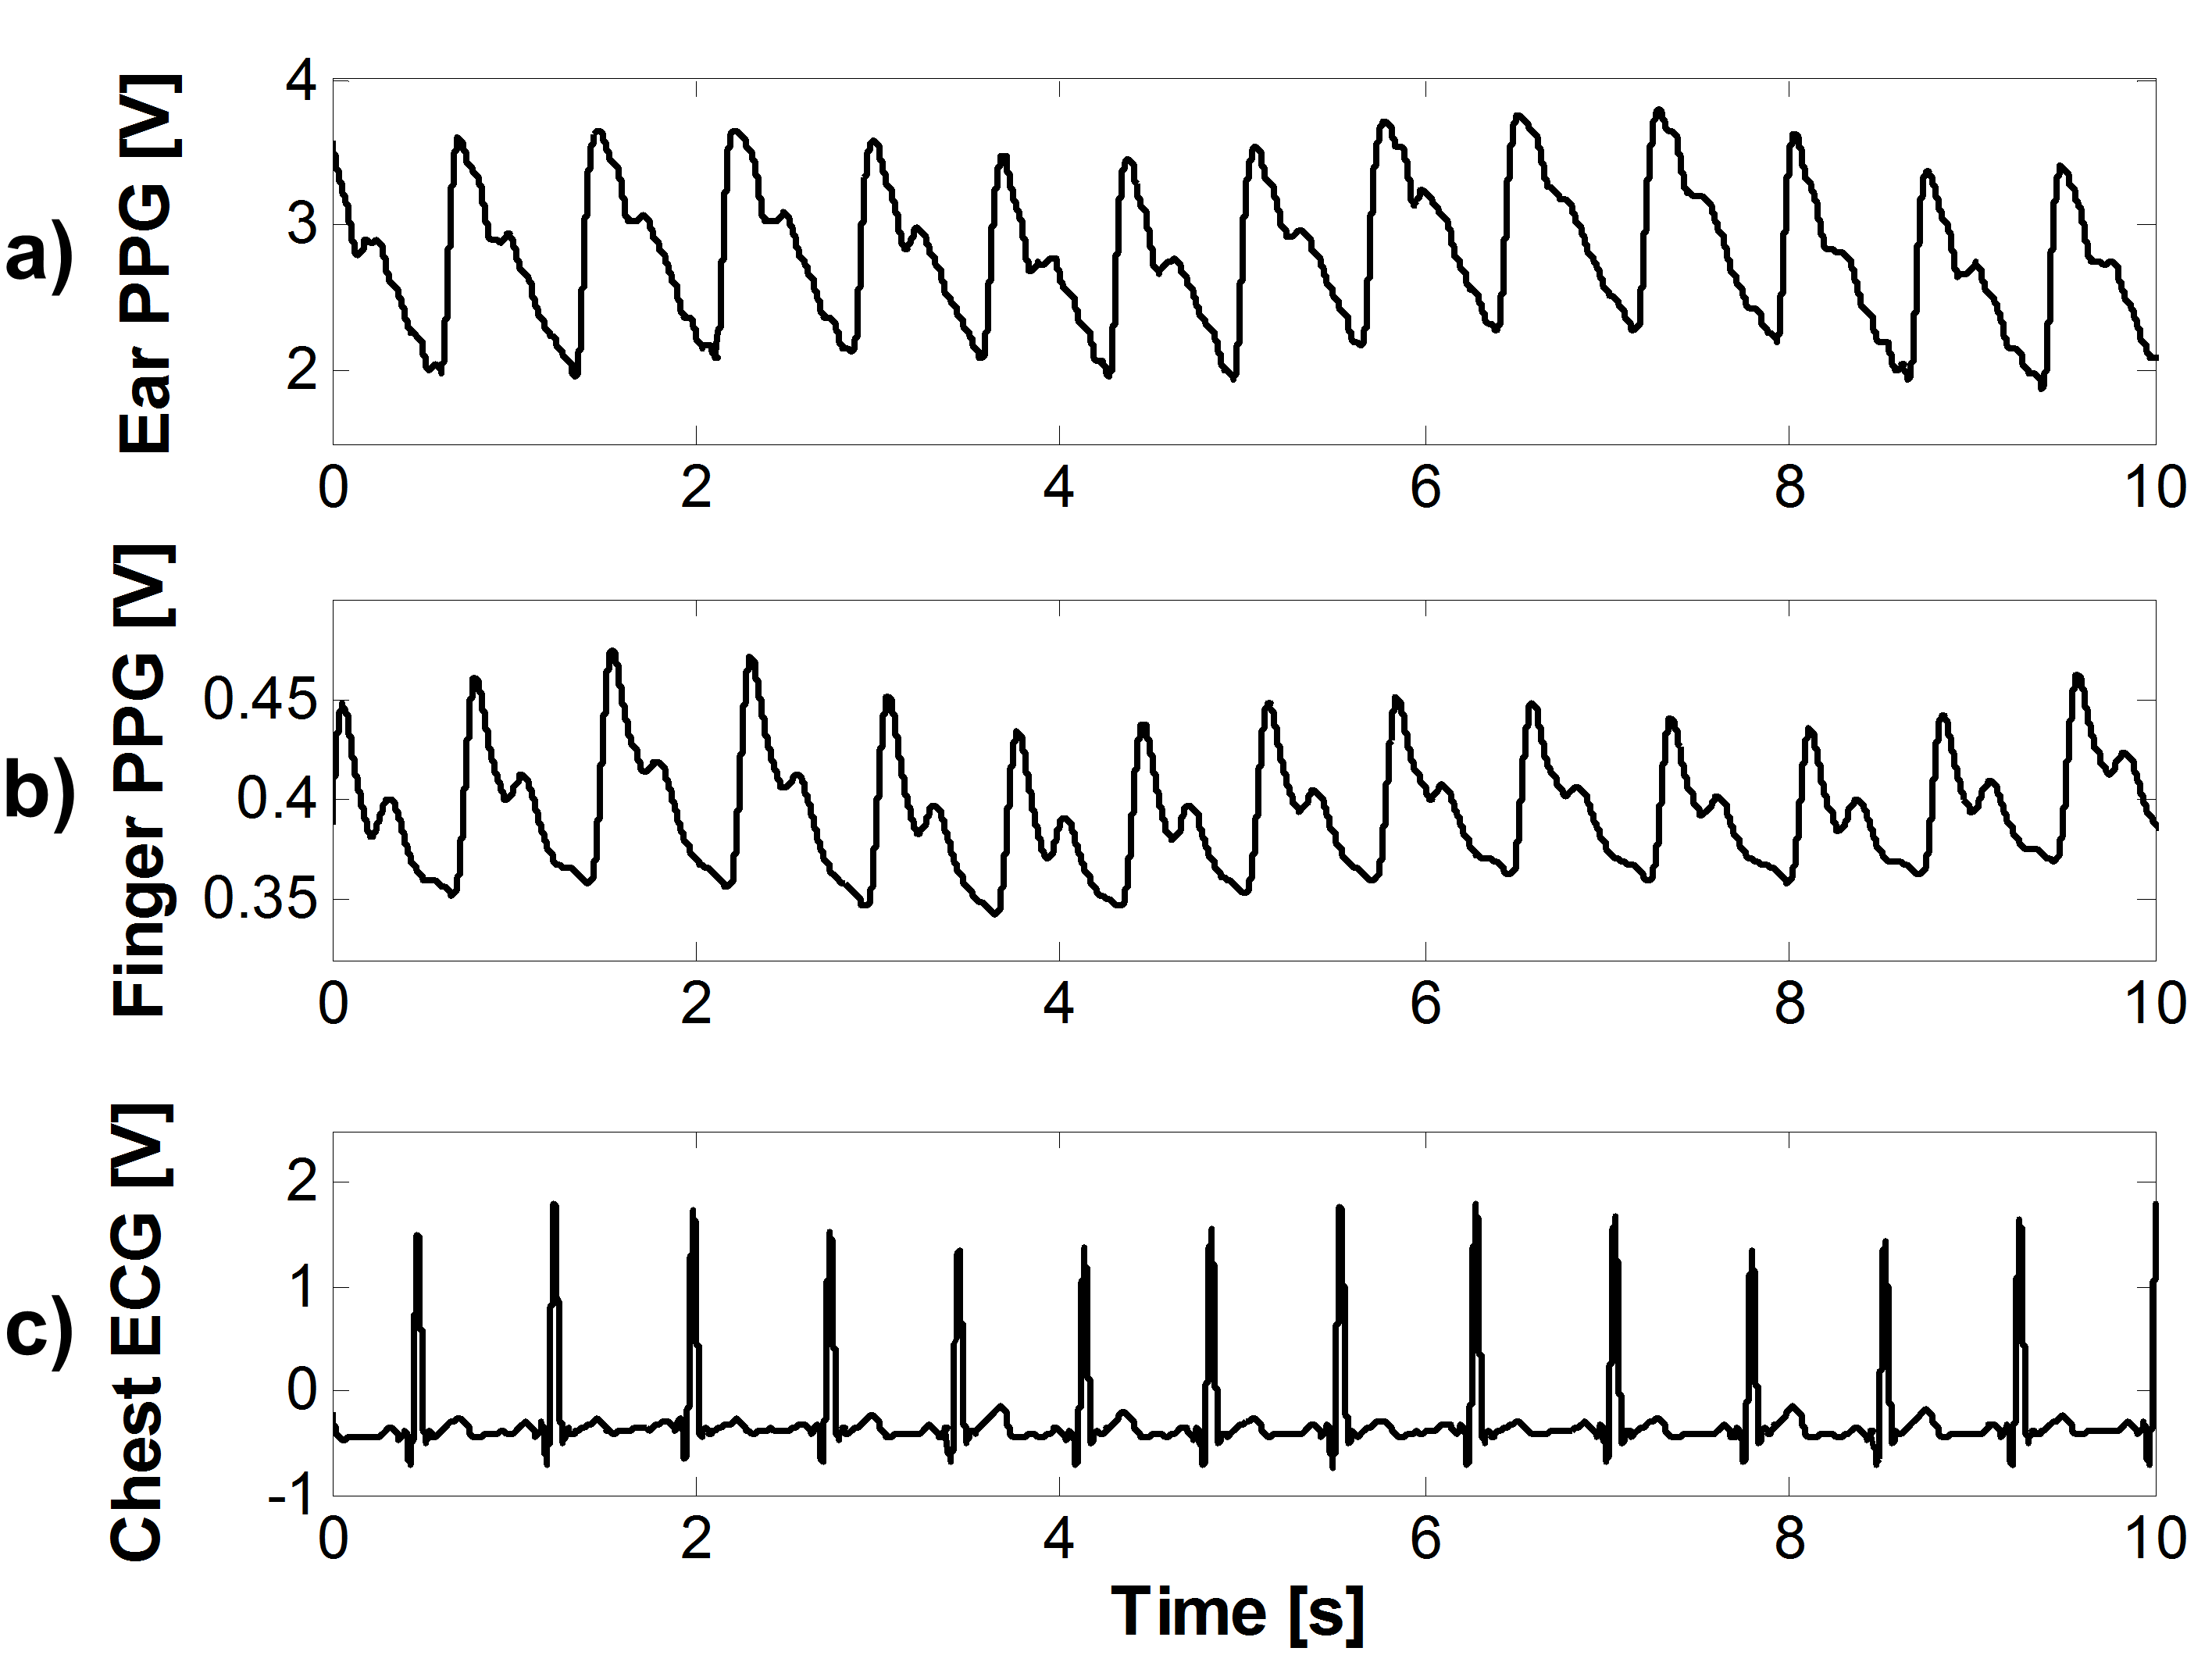
\includegraphics[scale=0.15]{figs/DaHe}
   \caption{Pulse oximetry diagram \citep{da2010ear}}
   \label{fig:DaHe}
\end{figure}

\cite{winokur2012wearable} developed a similar device that shines 660nm and 940nm light waves through tissue at the mastoid bone and collecting the reflected light with 4 photodetectors. A PPG front end conditioned the signals and their device sent the raw heart beat information to a PC through a radio connection. This is the same device that records ECG and is used to analyse heart intervals and mean blood pressure rather than heart rate.

\medskip
\cite{buskeheartbeat} proposed yet another location. They modified a pair of headphones to measure a transmission PPG from the concha. During the testing phase, the device showed an average heart rate accuracy of around 85\% when compared to an ECG.

\medskip
The \textit{cosinuss}$^{\circ}$ \textit{one}\textsuperscript \textregistered is a commercial device the monitors heart rate through the ear canal. The earpiece presses against the ear canal wall and records a PPG in reflection mode. It is marketed to athletes that want to monitor their bodies during exercise.

\begin{figure}[h]
   \centering
   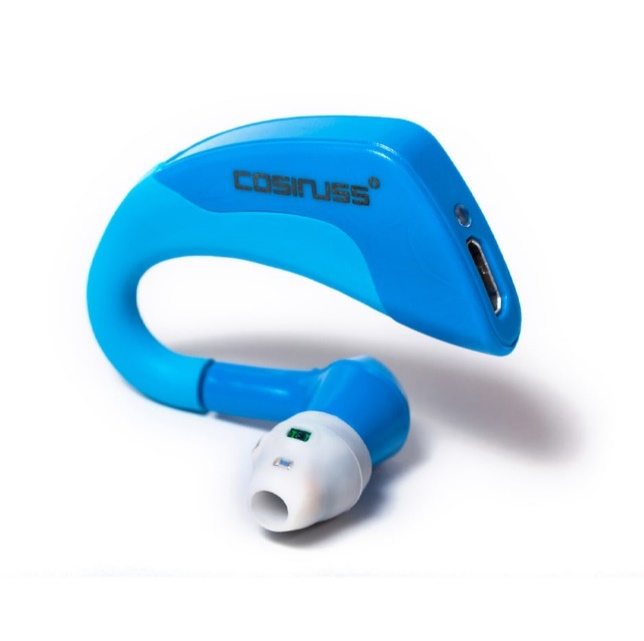
\includegraphics[scale=0.8]{figs/cosinuss}
   \caption{https://www.cosinuss.com/en/products/one}
   \label{fig:cosinuss}
\end{figure}


\subsection{Ballistocardiography}
BCG is the measurement of the mechanical effects of the beating heart on the body over time. Typically accelerometers or pressure sensors will be used to measure movement or forces on the surface of the body. BCG has been researched for use in ear heart rate extraction.

\medskip
In a wearable device proposed by \cite{da2010ear}, mechanical vibrations associated with heart rate are converted to electronic signals through capacitive sensing electrodes placed behind the ear. This method works by measuring the change in capacitance between the two electrodes as the distance between them changes due to heart rate vibrations.

\medskip
A study by \cite{winokur2012wearable} proposed measuring the head-to-foot axis recoil due to the blood-volume shift during cardiac ejection. This is done by placing an MEMS accelerometer behind the auricle. Due to the movement dependent method of operation this technology is extremely susceptible to motion artefacts and it can only be used during which the body is stationary.

\medskip
A variation of this technology is discussed in a article by \cite{park2015wearable}. They propose using a scissor shaped hinge mechanism in the ear canal that measures the change in the canal size due to the in-ear blood pulse waves. The mechanical movement is converted to an electrical signal through a piezoelectric film sensor. Figure \ref{fig:BCGsensor} shows an drawing of this device from Park's 2015 article.

\begin{figure}[h]
   \centering
   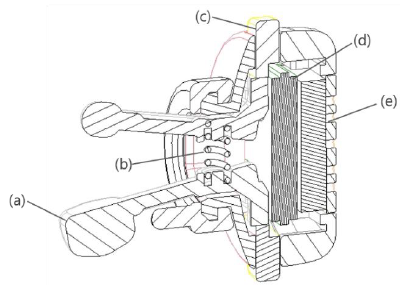
\includegraphics[scale=0.8]{figs/BCGsensor}
   \caption{Device to measure in ear pulse waves due to the heart beat \citep{park2015wearable}}
   \label{fig:BCGsensor}
\end{figure}

\subsection{Other Heart Rate Methods}
Electronic stethoscopes uses an microphone to record heart sounds. The hears makes a distinct series of sounds during the cardiac cycle due to blood turbulence and the shutting of heart valves. The period of this sound series can be used to determine heart rate and does not require skin-contact.

\medskip
A Doppler flow-meter can be used to detect the alternating blood current component in near-surface arteries. This component is synchronised to the heart rate frequency. The device can use ultrasound, microwaves of light to achieve the Doppler shift.

\section{Respiratory Rate}
Unlike the other medical signs, a person cannot measure his or her own respiratory rate. As soon as a person is consciously thinking about respiration, breathing usually slows. Measuring needs to happen while the person's thoughts are otherwise occupied. Therefore, a continuous measuring method are preferred. Typically, a nasal mask or chest strap will be used to measure respiration. 

\subsection{Respiratory Rate Ear Sensors}
Ear located devices that extract respiration information are rare, but some literature sources are available.

\medskip
\cite{goverdovsky2016hearables} tested an ear probe with two embedded microphones. The microphones could detect the sound created by turbulence in the airways for breathing rates higher than 12 breaths per minute. Figure \ref{fig:BreathingSound} shows a plot of the normalised sound amplitude at two different breathing rates. Variation during breathing can be seen in both recordings.

\begin{figure}[h]
   \centering
   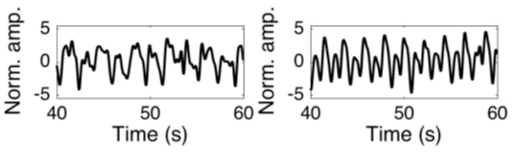
\includegraphics[scale=0.8]{figs/BreathingSound}
   \caption{Breathing detected through microphones inside the ear canal \citep{goverdovsky2016hearables}}
   \label{fig:BreathingSound}
\end{figure}

\cite{da2010ear} did extensive research on the ear as a location for medical sign monitoring. They extracted respiratory rate from baseline oscillations in a BCG signal recorded by capacitive electrodes placed behind the ear. Mechanical movement is converted to electrical signals by these electrodes. Therefore, the movement of the head due to respiration is seen on the BCG as baseline oscillations, Figure \ref{fig:BCGbreathing}.

\begin{figure}[h]
   \centering
   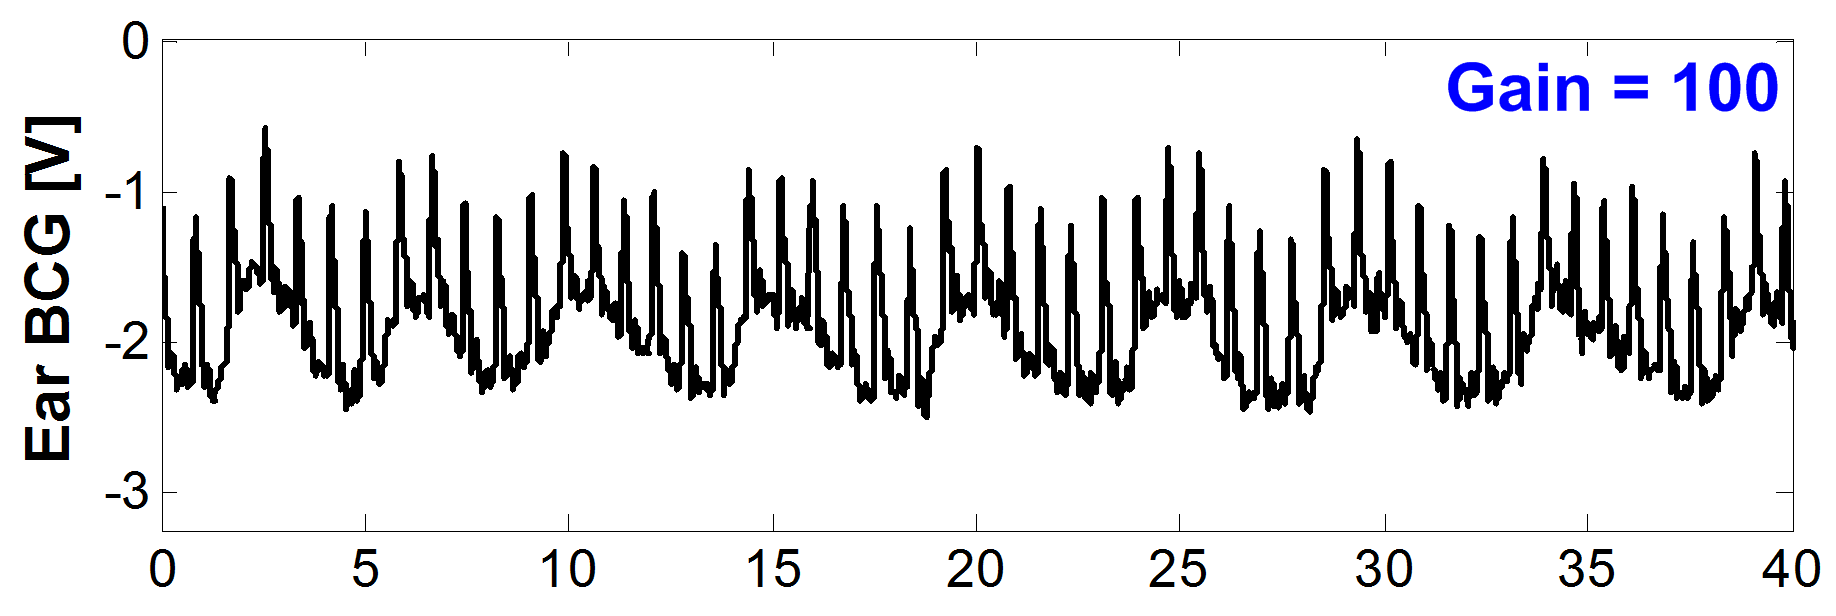
\includegraphics[scale=0.3]{figs/BCGbreathing}
   \caption{Baseline osculations in behind the ear BCG due to breathing \citep{da2010ear}}
   \label{fig:BCGbreathing}
\end{figure}

\subsection{Respiratory related Heart Rate Characteristics}
A different approach is to extract respiratory rate by looking at the heart rate. A PPG signal contains three distinct respiratory related characteristics: amplitude modulation (AM), respiratory-induced intensity variation (RIIV) and frequency modulation \citep{johansson2003neural}.

\medskip
Amplitude modulation is due to blood pressure changes during the respiratory cycle called Pulsus Paradoxus. RIIV is chances in the volume of the dermis and subcutaneous capillary bed. It is visible as baseline variation in the PPG signal.  Frequency modulation of the heart rate synchronised to respiration rate, called respiratory sinus arrhythmia (RSA).

\medskip
RSA can also be detected in ECG, but differ from the fluctuations seen in chest ECG, due to electrodes movement relative to the heart and changes in chest impedance during the respiratory cycle \citep{moody1986clinical}. These fluctuations cannot be detected in the ear. RSA is observed as baseline oscillation in heart rate in synchrony with the respiratory rate. Heart rate increase during inspiration and a decrease during expiration \citep{yasuma2004_RSA}. According to a study done by \cite{stratton2003effects}, the variation in heart rate due to RSA is higher in younger test subjects with 74\% increase in children vs. 52\% increase in adults.

\medskip
Research was been done to develop algorithms to utilise these characteristics to extract respiratory rate from PPG signals. \cite{clifton2007measurement} used wavelet analysis, achieved a respiratory rate accurate to within 1 breath per minute and \cite{leonard2006fully} documented a respiratory rate error of 7.9\%. \cite{johansson2003neural} developed two neural network algorithms that uses the different respiratory related characteristics of PPG signals to detect breaths. Table \ref{table:RRC} shows the results of the best algorithm.

\begin{table}
\centering
\caption{Results of the respiratory rate extraction through neural networks \citep{johansson2003neural}}
\begin{tabular}{P{5cm}P{3cm}P{3cm}}
 \hline
 Respiratory Related Characteristics & False Positive (\%) & False Negative (\%) \\ 
 \hline
 RSA  	& 	3.7 	& 	6.9 \\  
 AM 	& 	5.2 	& 	4.7 \\
 RIIV 	&	5.2		&	5.9 \\
 \hline
\end{tabular}
\label{table:RRC}
\end{table}


\section{Blood Oxygen Saturation}
Oxygen saturation can be measured by means of an arterial blood gas test resulting an arterial oxygen saturation reading. This requires drawing a blood sample for testing and therefore is not relevant to this study. An alternative method is pulse oximetry. This method estimates peripheral capillary oxygen saturation, $SpO_2$, through the spectrophotometric analysis of PPG signals captured at two different wavelengths. This is a clinically excepted estimation of the arterial oxygen saturation.

\subsection{Pulse Oximetry Theory}
Blood oxygen saturation estimation through pulse oximetry relies on the different adsorption spectra of oxyhaemoglobin and deoxyhaemoglobin. Figure \ref{fig:AbsorptionSpectra} shows the absorption spectra of oxy- and deoxyhaemoglobin. 

\medskip
\begin{figure}
   \centering
   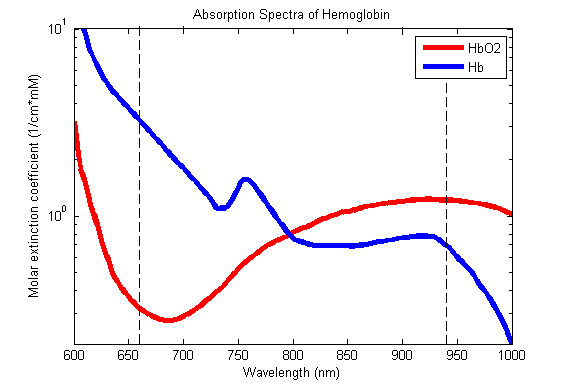
\includegraphics[scale=0.8]{figs/AbsorptionSpectra_Edit}
   \caption{Absorption spectra of oxy- and deoxyhemoglobin}
   \label{fig:AbsorptionSpectra}
\end{figure}

It can be noted that deoxyhaemoglobin has a significantly higher absorption of red light while oxyhaemoglobin has a slightly higher absorption of infrared light.

\medskip
According to Beers law, the amount of light absorbed by a dissolved substance is proportional to its concentration \citep{lambertANDbeer}. Therefore, oxygenated blood (with a higher concentration of oxyhaemoglobin) will absorb more infrared light and reflect more red light. Whereas deoxygenated blood (with a higher concentration of deoxyhaemoglobin) will absorb more red light and reflect more infrared light. This explains why oxygenated blood appears bright red, while deoxygenated blood is a darker shade of red.

\medskip
Red and infrared light are shined into the peripheral tissue and the light reflected or transmitted is measured for both wavelengths. Literature and commercial devices usually uses wavelengths of 660 nm (red) and 940 nm (near infrared) \citep{tytler1986nellcor} \citep{ti2012datasheet} \citep{bagha2011real} \citep{bheema2013spo2} \citep{duun2007novel}. The ratio of reflected or transmitted light is unique to a certain level of blood oxygen saturation and is used to estimate blood oxygen saturation.

\medskip
The Beer-Lambert law describes the absorption of a specific wavelength of light by a substance in a homogeneous solution \citep{bagha2011real}. 

$$A=\varepsilon cL=ln\left( \frac{I_o}{I}\right) $$
$$I=I_o e^{-\varepsilon _\lambda cL}$$

\medskip
Where $A$ is the dimensionless adsorption, $\varepsilon$ is the wavelength dependant molar absorptivity, $c$ is the concentration of the substance and $L$ is the path length the light needs to travel through the substance. $I_o$ is the intensity of the light entering the solution and $I$ is the intensity of light passing though the solution.

\medskip
When applying this law to measuring $O_2$ saturation, a concentration ratio can be calculated. Factoring out $L$, $I_o$, and the constants in $\varepsilon$, the ration can be written as:

$$R=\frac{log\left( I_{red} \right)\cdot\lambda _{red}}{log\left( I_{ir} \right)\cdot\lambda _{ir}}$$

\medskip
Where $I$ is the light intensities and $\lambda$ is the wavelength \citep{ti2012datasheet}.  Red and infrared light sources are alternated and intensity measurements are made for both separately.

\medskip
In practice, a different modulated relationship is used to compensate for the different DC absorption between patients \citep{konig1998reflectance} \citep{duun2007novel} \citep{bheema2013spo2}   \citep{bagha2011real}  \citep{nitzan2014calibration} \citep{ti2012application}

$$R = \frac{\left(\frac{AC}{DC}\right)\textsubscript{red}}{\left(\frac{AC}{DC}\right)\textsubscript{IR}} $$

\medskip
This ensures that the $O_2$ saturation of only the arterial blood is calculated. The ration can be checked against an empirical determined curve. The standard formula for this curve is found in literature as \% $SpO_2  = 110-25R$, \citep{ti2012application} but it can vary from device to device.

\medskip
As mentioned, $SpO_2$ can be calculated using reflected or transmitted light. Light that is not absorbed or scattered by tissue can be either reflected, or transmitted. Thus, both reflected and transmitted light is proportional to the mount of light absorbed. Transmittance mode pulse oximeters are more common, but their use is restricted to parts of the body that will allow for light to pass through, like a fingertip or earlobe.

\medskip
A big challenge to conventional pulse oximeters is noise due to movement \citep{spo2Motion}.

\subsection{Work done by others in ear pulse oximetry}
Standard locations for pulse oximetry includes the fingertip, earlobe, ankle and forehead. A study comparing fingertip and earlobe pulse oximetry to an arterial blood gas test found that finger pulse oximetry differed by a mean of -0,71\% and earlobe pulse oximetry differed by a mean of +4.2\% \citep{olive2016comparison}. Literature and commercial wearable pulse oximeters typically utilise a finger clip to measuring $SpO_2$ \citep{watthanawisuth2010wireless} \citep{pujary2003photodetector} \citep{huang2014novel} \citep{khalifa2014development}. This location is not ideal for continuous monitoring and is especially susceptible to motion artefacts. Although the fingertip location is not of interest to this study, the literature is still reviewed for similar principals can be applies to ear pulse oximetry.

\medskip
Ear lobe pulse oximetry usually done through a sensor that clips to the ear lobe, which is attached to a stationary device. Wearable ear pulse oximetry, is still novel and not well covered in literature. There are some patients filled for such devices (US 20050177034 A1) (US 4086915 A) (US 3412729 A) (US 6556852 B1) and commercial devices like but little academic material is available.

\medskip
A study done by \citep{aziz2006pervasive} tested a wireless earlobe-mounted pulse oximeter on a group of subjects. Subjects were tested while sitting, walking and running. During the sitting and walking phases they recorded an SpO2 reading of above 95\%, which is \enquote{as expected} according to them. But during the running phase they could not obtain any accurate reading. 

\medskip
During running, they could not take an $SpO_2$ reading, but Literature on ear PPG, only uses infrared light to determine heart rate. Theoretically, infrared light can be added in the same way to produce and red PPG and a R value can be calculated to estimate $SpO_2$.

\medskip
Pulse oximetry patch

\section{Electrical Brain Activity}
